\documentclass[10pt]{report}
%\usepackage{fullpage}
\usepackage{graphicx}   % if you want to include graphics files
\usepackage{subfigure}
\usepackage{setspace}
\usepackage{amsxtra}
\usepackage{bm}

\usepackage{amsmath}
\usepackage{amsfonts}
\usepackage{amssymb}
\usepackage{multirow}
\usepackage{algorithmic}
\usepackage{algorithm}

% graphics path
\graphicspath{{Figs/}}
%\usepackage{rotating}

%turns all margins to 1in
\addtolength{\oddsidemargin}{-.875in}
\addtolength{\evensidemargin}{-.875in}
\addtolength{\textwidth}{1.75in}

\addtolength{\topmargin}{-.875in}
\addtolength{\textheight}{1.75in}

\DeclareMathOperator{\sgn}{sgn} 
\setcounter{secnumdepth}{2}
\author{John Swoboda}
\title{\textbf{Incoherent Scatter Radar Simulator}}

\begin{document}
\maketitle

\chapter{Introduction}

This report covers the physics, and signal processing used to create the incoherent scatter radar (ISR) simulator that is in the code base. The simulator was developed to make synthetic data that one could use to create different processing algorithms and methods while having a known input or "truth" data. This simulator will take plasma fields of plasma parameters, create IQ from these parameters and then process that data to the point where it can estimate the input plasma parameters.

The need to create a full 3-dimensional software package was necessitated by the desire to explore the utility of the new phased array radar systems and their ability to measure 3-D fields of plasma parameters. This desire to understand the measurement capabilities of electronically scanned ISR lead to the following publication \cite{RDS:RDS20236} where this software package was usedto create reconstructions of 3-D fields of plasma parameters.

The software itself has been developed in such a way that the code mirrors the processing. Overall there are three main classes: 

\begin{itemize} 
\item IonoContainer - A container class that holds information on the ionosphere or auto correlation functions (ACFs)/spectrums, both intrinsic and estimated.

\item RadarDataFile - A class that holds and operates on the radar data to create estimates of the autocorrelation function. The class takes files containing ISR spectrums and then creates ISR data and as a final step outputs instances of the IonoContainer class that holds estimates of the plasma ACF.

\item FitterMethodsGen - A class that applies the fitter to the data and outputs an instance of IonoContainer with the measured parameters. 
\end{itemize}

The overall flow can be seen in figure \ref{fig:swflow}, where  $\Theta$ is the plasma parameters $ g(\Theta)$ is a function that turns the plasma parameters to ISR spectrums, $ \mathbf{r}$ is the spectrums/ACFs for each point of time and space, $ \mathbf{Lr}$ is the radar's operator on the spectrums/ACFs, $ \rho$ is the measured ACFs from the radar and lastly $ \hat{\Theta}$ is the estimates of plasma parameters from $ \rho$ after least squares fitting.

\begin{figure}[!h]
\centering
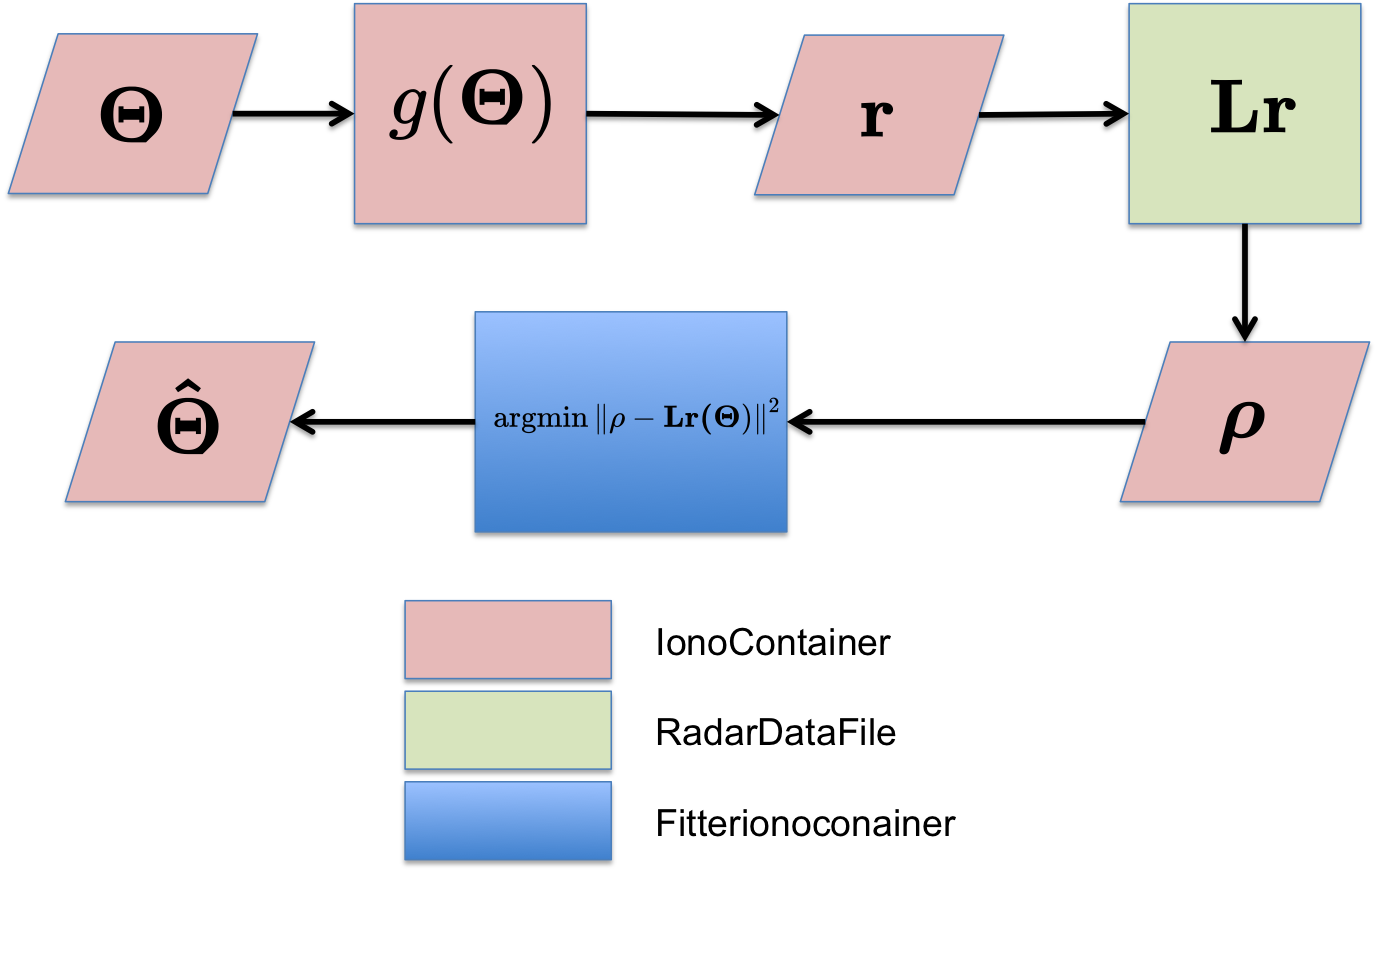
\includegraphics[width=6.0in]{softwareflowandmath}
% where an .eps filename suffix will be assumed under latex, 
% and a .pdf suffix will be assumed for pdflatex; or what has been declared
% via \DeclareGraphicsExtensions.
\caption{Software flow diagram}
\label{fig:swflow}
\end{figure}

This report is broken up in to the following chapters. The next chapter will cover the method to calculate the ISR spectrum. There are a number of publications on this including \cite{dougherty:farley1960, hagfors1971, sheffield2010} that cover this area but we focus on the treatment found in \cite{kudeki:milla:1}. Next the method to form the ISR data will be shown, this will include the signal processing steps taken to create the data. The processing of the data from estimating the lags to fitting the plasma parameters will then be covered. We will focus on methods for long pulse but we will show where this differentiates when using other waveforms such as alternating codes and Barker codes. Lastly we will show examples of the output of the ISR simulator at a number of different spots in the processing chain.
 
\chapter{ISR Spectrum}
\section*{Overview}

This is a description of the ISR spectrum process describes the mathematical basis for the software code base ISRSpectrum. It is based off of the development in  \cite{kudeki:milla:1} and \cite{Kudeki:2006kx} to form a spectrum.

\section*{Determining Spectra}
The first step comes from \cite{kudeki:milla:1} where a lumped circuit model is used to describe the spectrum. In it the independent thermal fluctuations of each species of ions and electrons are treated as current sources and the macroscopic conductances are treated as discrete components. The electric field $E$ impinged from the radar acts as a voltage. This lumped circuit model, seen in Figure \ref{fig:circuit}, is derived is taking the scalar component of Ampere's law in the direction of $\mathbf{k}$.  

\begin{equation}
\label{eq:ampere}
-j\mathbf{k} \times \mathbf{H} = \mathbf{J} +j\omega \epsilon_0 \mathbf{E},
\end{equation}

\noindent which then yields,

\begin{equation} 
\label{eq:ampscaler}
0=(\sigma_i +\sigma_e)E +\frac{\omega}{k}e(n_{ti}-n_{te}) +j\omega \epsilon_0 E.
\end{equation}

\begin{figure}[!h]
\centering
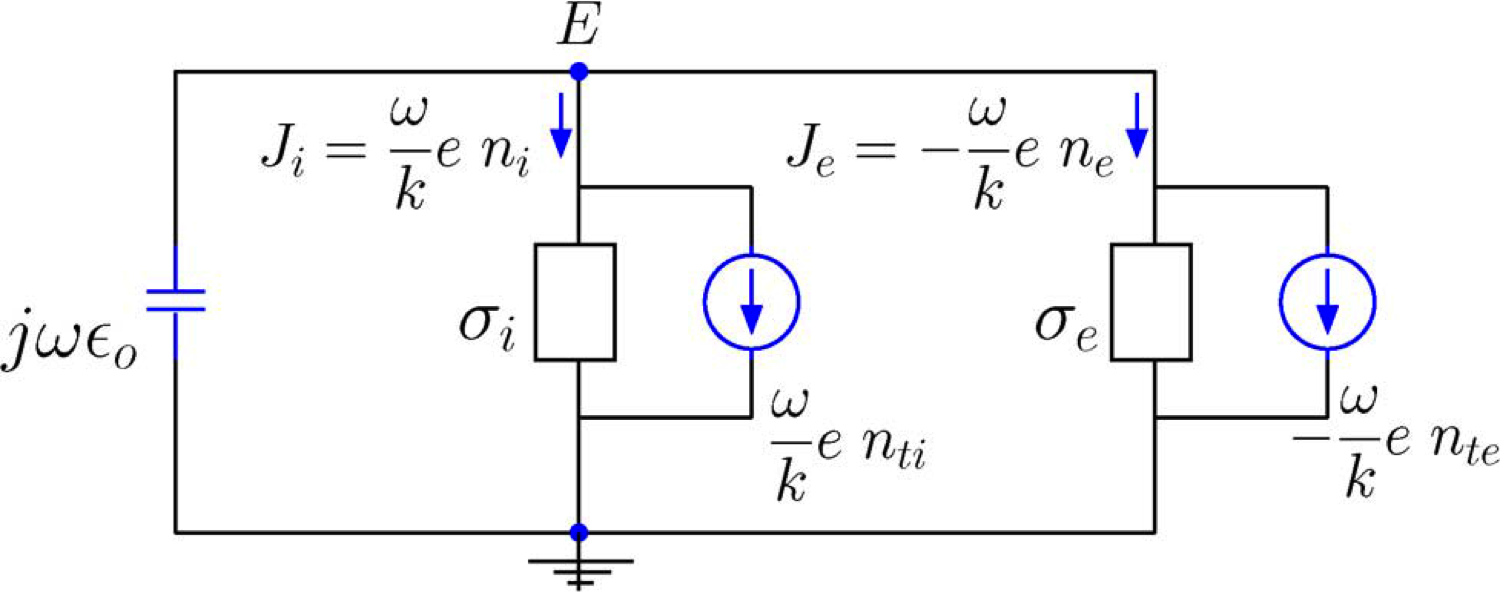
\includegraphics[width=3.0in]{circuit}
% where an .eps filename suffix will be assumed under latex, 
% and a .pdf suffix will be assumed for pdflatex; or what has been declared
% via \DeclareGraphicsExtensions.
\caption{Lumped circuit model seen in  \cite{kudeki:milla:1}.}
\label{fig:circuit}
\end{figure}

\noindent Using the electron current expression, $-\omega k^{-1}en_e = E\sigma_e -\omega k^{-1}en_{te}$, these equations can be rearranged to solve for $n_e$, 

\begin{equation}
\label{eq:neeq}
n_e(\mathbf{k},\omega) =  \frac{(j\omega\epsilon_0 + \sigma_i) n_{te}(\mathbf{k},\omega)}{j\omega\epsilon_0 +\sigma_e+\sigma_i} + \frac{\sigma_en_{ti}(\mathbf{k},\omega)}{j\omega\epsilon_0 +\sigma_e+\sigma_i}.
\end{equation}

\noindent To determine the power spectrum we square and average Equation \ref{eq:neeq} taking into account that the terms $n_{te}$ and $n_{ti}$ are independent of one and other we result in the following
\begin{equation}
\label{mainspeceq}
\langle \left|n_e(\mathbf{k},\omega)\right|^2\rangle = \frac{|j\omega\epsilon_0 + \sigma_i|^2 \langle |n_{te}(\mathbf{k},\omega)|^2\rangle}{|j\omega\epsilon_0 +\sigma_e+\sigma_i|^2} + \frac{| \sigma_e|^2 \langle |n_{ti}(\mathbf{k},\omega)|^2\rangle}{|j\omega\epsilon_0 +\sigma_e+\sigma_i|^2}.
\end{equation}

We can generalize them for multiple ion species by simply summing over the thermal fluctuations and conductances in Equation \ref{eq:ampscaler},

\begin{equation} 
\label{eq:ampscalersum}
0=\left(\displaystyle \sum_k^K\sigma_{ik} +\sigma_e\right)E +\frac{\omega}{k}e\left(\sum_k^Kn_{tik}-n_{te}\right) +j\omega \epsilon_0 E.
\end{equation}

\noindent This then augments the power spectrum in Equation \ref{mainspeceq} to the following

\begin{equation}
\label{eq:sumspeceq}
\displaystyle \langle \left|n_e(\mathbf{k},\omega)\right|^2\rangle = \frac{\left|j\omega\epsilon_0 +  \sum_k^K\sigma_{ik} \right|^2 \langle |n_{te}(\mathbf{k},\omega)|^2\rangle}{\left|j\omega\epsilon_0 +\sigma_e+ \sum_k^K\sigma_{ik} \right|^2} + \frac{| \sigma_e|^2 \left \langle \left|\sum_k^Kn_{tik}(\mathbf{k},\omega)\right|^2\right\rangle}{\left|j\omega\epsilon_0 +\sigma_e+ \sum_k^K\sigma_{ik} \right|^2}.
\end{equation}

%%%%%%%%%%%%%%%%%%%%%%%%%%%%%%%%%%%%%%%%%%%%%%%%%%%%%%%%%%%%%%%%%%%%%%
\section*{Gordeyeve Integrals}
The power spectrum of the thermal fluctuation for each species $s$ can be determined by the following,

\begin{equation}
\label{eq:thermalfl}
\frac{\langle|n_{ts}(\mathbf{k},\omega)|^2\rangle}{N_0} = 2\text{Re}\{J_s(\omega_s)\},
\end{equation}

\noindent where $N_s$ is the average density for the species.  Also the conductance for each species $s$ can be determine from the following,

\begin{equation}
\label{eq:cond}
\frac{\sigma_{s}(\mathbf{k},\omega)}{j\omega\epsilon_0} = \frac{1-j\omega_s J_s(\omega_s)}{k^2\lambda_s^2}
\end{equation}

\noindent where $\omega_s \equiv \omega-\mathbf{k}\cdot\mathbf{V}_s $ is the Doppler shifted frequency and $\lambda_s \equiv \sqrt{\frac{\epsilon_0 KT_s}{N_s q_s^2}}$ is the Debye length for each species.

The $J_s$ terms can be represented as follows

\begin{equation}
\label{eq:gord}
J_s(\omega)\equiv \int_0^\infty \langle e^{j\mathbf{k}\cdot\Delta \mathbf{r}_s}\rangle e^{j\omega\tau}d\tau
\end{equation}

\noindent These terms are known as Gordeyeve integrals, which are the one sided Fourier transforms of the characteristic functions of the particle displacements $\langle e^{j\mathbf{k}\cdot\Delta\mathbf{r}_s}\rangle$.  

The particle displacement function can change depending on magnetic field and collisionality of the plasma. For the high latitude F-region in the ionosphere a case of general importance is one of a non-magnitized and collision less plasma, where $\Delta\mathbf{r} = \mathbf{v}\tau$ where $\tau$ is the time interval. Assuming a Maxwellian the PDF of one dimensional displacement is

\begin{equation}
\label{eq:pdfr}
f(\Delta r) = \frac{1}{\sqrt{2\pi \langle r^2 \rangle}}e^{\frac{-\Delta r^2}{2\langle r^2\rangle}}.
\end{equation}
 
\noindent The variance term $\langle r^2 \rangle$ can be represented as
\begin{equation}
\label{eq:var}
\langle r^2 \rangle = \langle v^2 \rangle \tau^2 = \frac{KT_s}{m_s} \tau^2
\end{equation}
 \noindent where $T_s$ is the temperature of the species, $K$ is Boltzmans constant and $m_s$ is the mass of the species in kg. To simplify notation like in \cite{kudeki:milla:1}, we will refer to $\sqrt{KT_s/m_s}$ as $C$. Which yields the following single particle ACF,
 
 \begin{equation}
\label{eq:pdfall}
\langle e^{j\mathbf{k}\cdot\Delta \mathbf{r}}\rangle= e^{-\frac{1}{2}k^2C^2 \tau^2}.
\end{equation}
 
 To model collisions we use the term $\nu$ as the collision frequency for the species. If $\nu<<kC$ then \ref{eq:pdfall} can be used as the single particle ACF. If not the following must be used.
 
 \begin{equation}
 \label{eq:colspacf}
 \langle e^{j\mathbf{k}\cdot\Delta \mathbf{r}}\rangle = e^{-\frac{k^2C^2}{\nu^2}\left( \nu \tau-1+e^{-\nu\tau}\right)}
 \end{equation}
 
Lastly if one is to add a magnetic field to the equations the single particle ACFs must now take into a account the orientation of the magnetic field. The authors of \cite{kudeki:milla:1} use the convention of breaking up the Bragg vector $\mathbf{k}$ into two components, one parallel to the magnetic field, $k_{\parallel}$ and one perpendicular,$k_{\perp}$, as such, $\mathbf{k}= \hat{b}k_{\parallel}+\hat{p}k_{\perp}$. This yields the following formulation for the single particle ACF,

 \begin{equation}
\label{eq:pdfmag}
\langle e^{j\mathbf{k}\cdot\Delta \mathbf{r}}\rangle= e^{-\frac{1}{2}k_{\parallel}^2C^2 \tau^2}\times e^{-\frac{2k_{\perp}^2C^2}{\Omega^2} \sin^2(\Omega\tau/2)},
\end{equation}

\noindent where the gyro frequency is $\Omega = qB/m$This formulation neglects the effects of collisions which if taken into account yields the following single particle ACF,

\begin{equation}
\label{eq:colspacf}
\langle e^{j\mathbf{k}\cdot\Delta \mathbf{r}}\rangle = e^{-\frac{k_\parallel^2C^2}{\nu^2}\left( \nu \tau-1+e^{-\nu\tau}\right)}\times e^{-\frac{k_\perp^2C^2}{\nu^2+\Omega^2}\left(\cos(2\gamma) + \nu \tau-e^{-\nu\tau}\cos(\Omega\tau-2\gamma)\right)},
\end{equation}
 
\noindent where $\gamma = \tan^{-1}(\nu\Omega)$. The for the case with the magnetic field as one gets closer to being fulling perpendicular to $\mathbf{B}$ the single particle ACFs become much more narrow band, to the point of becoming delta functions in the frequency space. It is necessary to use other methods beyond numerical integration to determine the Gordeyeve Integrals. The authors of \cite{kudeki:milla:2} get around this problem by making a PIC code to determine the particle statistics. 


%%%%%%%%%%%%%%%%%%%%%%%%%%%%%%%%%%%%%%%%%%%%%%%%%%%%%%%%%%%%%%%%%%%%%%
 \section*{Computational Considerations}
One of the main challenges to calculating the ISR spectrums is calculating the Gordeyeve integrals. The case with no collisions or magnetic fields can be done analytically using Dawsons integral. This can be done using the identity

\begin{equation}
\label{eq:daw1}
jZ(\theta) = \int_0^{\infty} e^{-j\theta t}e^{-\frac{t^2}{4}}dt = \sqrt{\pi}e^{-\theta^2}-j2e^{-\theta^2}\int_0^\theta e^{t^2}dt.
\end{equation}

\noindent Using the terms found in Equation \ref{eq:pdfall}, $\theta=\omega_s/\left(\sqrt{2}kC\right)$ and $t=\sqrt{2}kC\tau$.

For other cases where analytical calculation is not possible a numerical integration scheme from \cite{Ooi:2007jx} is used. It is also possible to use a Chirp-z based algorithm that is shown in \cite{Li:1991gr} from the experiences of the author the first technique converges faster. The technique used in \cite{Ooi:2007jx} changes the variable of integration for integrals of the following form,

\begin{equation}
\label{eq:Sommer}
I=\int_a^b f(z) dz.
\end{equation}

\noindent The technique changes the variable $z$ in the following way,

\begin{equation}
\label{eq:newz}
z = \frac{1}{2}(a+b)+\frac{1}{2} (b-a)\text{Erf}(g(t)),
\end{equation}

\noindent where $g(t)$ is a function that is choosen so  $g(t)\rightarrow\pm \infty$ as $t\rightarrow\pm \infty$ and $Erf(u)$ is 
\begin{equation}
\label{eq:erf1}
\text{Erf}(u) = \frac{2}{\sqrt{\pi}}\int_0^u e^{-t^2}dt.
\end{equation}

\noindent Discretizing and changing variables the integral in Equation \ref{eq:Sommer} becomes the following sum

\begin{equation}
\label{eq:erfsum1}
I=\displaystyle \sum_{n=-N}^N A_nf\left( \frac{1}{2}(a+b)+\frac{1}{2} (b-a)\text{Erf}(g(nh))\right)
\end{equation}

\noindent where,
\begin{equation}
\label{eq:anterm}
A_n = g'(nh)e^{-g(nh)^2}.
\end{equation}

\noindent Like in \cite{Ooi:2007jx}, $g(nh) = \sinh (nh)$ and the grid spacing $h$ is the following,

\begin{equation}
\label{eq:hterm}
h = \frac{1}{N}\ln(1.05\sqrt{2}N).
\end{equation} 


Lastly to avoid cases of divid by zero errors the main equations have to be rearrange slightly. First off because some ion species could have zero density Equation \ref{eq:cond} uses the Debye length of the electron species,$\lambda_e$ as follows

\begin{equation}
\label{eq:condnew}
\frac{\sigma_{s}(\mathbf{k},\omega)}{j\omega\epsilon_0} = \frac{1-j\omega_s J_s(\omega_s)}{k^2\lambda_e} \left(\frac{q_sT_eN_s}{q_eT_sN_e}\right).
\end{equation}

Also, to avoid having to more calculations then necessary the $j\omega\epsilon_0$. terms of Equation \ref{eq:sumspeceq} are moved around. Thus it becomes,

\begin{equation}
\label{eq:sumspeceqfinal}
\displaystyle \langle \left|n_e(\mathbf{k},\omega)\right|^2\rangle =  \frac{\left|1 +  \sum_k^K\frac{\sigma_{ik}}{j\omega\epsilon_0} \right|^2 \langle |n_{te}(\mathbf{k},\omega)|^2\rangle}{\left|1 +\frac{\sigma_e+ \sum_k^K\sigma_{ik}}{j\omega\epsilon_0} \right|^2} + \frac{\left| \frac{\sigma_e}{j\omega\epsilon_0} \right|^2\left \langle \left|\sum_k^Kn_{tik}(\mathbf{k},\omega)\right|^2\right\rangle}{\left|1 +\frac{\sigma_e+ \sum_k^K\sigma_{ik}}{j\omega\epsilon_0} \right|^2}.
\end{equation}

\section*{Examples}
We can see in Figure \ref{fig:diffspectrums} examples of ISR spectrums from different ISR systems. The spectrums were generated using the the parameters values $N_e=1e11$, $T_e=3000^o$K and $T_i=3000^o$K and the system parameter values seen in Table \ref{tab:ISRsys}. The ion acoustic frequency$f_{ia}$ for each system with the following plasma parameters its wavelength $\lambda$ was calculated using the following formula,

\begin{equation}
\label{eq:iaf}
f_{ia} = \frac{\lambda}{2}\sqrt{\frac{k_bT_e +k_b\gamma_iT_i}{M}},
\end{equation}

\noindent where $M$ is the ion mass in kg, $k_b$ is Botlzmann's constant and $\gamma_i$ is the adiabatic index which is set to 3 in all cases. In most of the cases the familiar double hump spectrum is visible. The only exception to this is Jicamarca, where the system's k-vector is very close to being perpendicular to the earths magnetic field. This also impacts the amount of time it takes to calculate the spectrum because as the k-vector gets closer to being perpendicular to magnetic field the Gordeyeve integral will take longer to converge.
\begin{figure}[!h]
\centering
\includegraphics[width=7.0in]{DifferentSystems}

\caption{Spectrums From Different ISR Systems}
\label{fig:diffspectrums}
\end{figure}


\begin{table}[!h]
\centering
\caption{ISR System Parameters}
\label{tab:ISRsys}
\begin{tabular}{lllll}
System Name & $f_0$ in MHz & $f_s$ in kHz & $\alpha$ in $^o$ &  \\
AMISR       & 449          & 50           & 70               &  \\
Sondrestrom & 1290         & 100          & 80               &  \\
Haystack    & 440          & 50           & 65               &  \\
Arecibo     & 430          & 50           & 45               &  \\
Jicamarca   & 50           & 10           & 1                & 
\end{tabular}
\end{table}
%%%%%%%%%%%%%%%%%%%%%%%%%%%%%%%%%%%%%%%%%%%Chapter 2%%%%%%%%%%%%%%%%%%%%%%%%%%%%%%%%%%%%%%%%%%%%%
\chapter{Data Creation}

\section*{Overview}
The goal of incoherent scatter radar is to measure plasma parameters by first estimating a power spectrum from the random fluctuations of the electron density in the ionosphere. In order to model the the return signal from an ISR a complex gaussian process with a correlation properties dictated by the plasma parameters is created. 
In this chapter the methods used to create the ISR data are detailed. The First the inputs will be covered, after which the signal processing procedures to make the base band IQ data will be shown.

\section*{Inputs}
The simulator takes as input a discretized set of ionosphere parameters in Cartesian coordinates and which can change with time. Each point in time and space has a set of parameters that allow it to make an ISR spectrum using the methods detailed in the previous chapter. The spectrums are then created so every point in space and time will have its own intrinsic ISR spectrum. The radar will then act on these spectrums as a linear operator and average them together in time and space using the beam patterns and pulse pattern. 

Using the fact that any spatial correlations between the electron density fluctuations will be on the order of the Debye length \cite{farley1969}, the intrinsic ISR spectrums will be first averaged over a resolution cell for the radar. 

\section*{Signal Processing}
The IQ data is created by taking a complex white Gaussian noise process and shaping the spectrum using a filter. Each point in space and time will have a separate noise plant and filter which is derived from the plasma and radar parameters parameters, like that seen in Figure \ref{fig:IQdiagram}. 
%The 3-D ISR simulator creates data by deriving a time filter from the autocorrelation functions and applying them to complex white Gaussian noise generators. Stating this in another way, every point in time and space has a noise plant and filter structure as in Figure \ref{fig:IQdiagram}. 
\begin{figure}[h!]
\centering
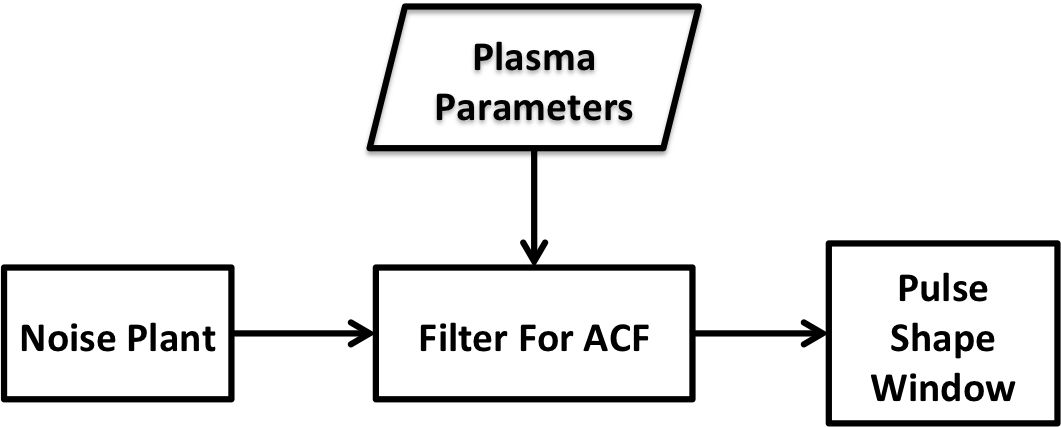
\includegraphics[width=4in]{diagrampart}
\caption{Diagram for I/Q simulator signal flow.}
\label{fig:IQdiagram}
\end{figure}

The radar samples the space in a spherical coordinate system with discrete range and beam positions. For each range gate and beam the different spectrums are averaged together together. In range this is simply a window the length of a range gate. Across the azimuth and elevation space the beam pattern for the system is used. In order to calculate the beam pattern for the AMISR system the method detailed in the appendix of \cite{RDS:RDS20236}. The entire process of the spatial sample is shown in the simplified diagram in Figure \ref{fig:beamdia}.


\begin{figure}[!t]
\centering
\includegraphics[width=2in]{beamsampling}
% where an .eps filename suffix will be assumed under latex, 
% and a .pdf suffix will be assumed for pdflatex; or what has been declared
% via \DeclareGraphicsExtensions.
\caption{Beam Sampling Diagram}
\label{fig:beamdia}
\end{figure}

Once the spectrum has been created the filter,$H_m(\omega)$, is created by simply taking the square root of the spectrum, $S_m(\omega | \: \bm{\theta})$

\begin{equation}
\label{eq1}
H_m(\omega) = \sqrt{S_m(\omega | \: \bm{\theta})}.
\end{equation}

\noindent The term $ \bm{\theta}$ refers to the different plasma and system parameters needed to make the spectrum. Complex white Gaussian noise  ($w(k)\sim CN(0,1)$) is then pushed though each of the filters and then windowed by the pulse creating the following:   

\begin{equation}
\label{eq2}
y_m (k)= s(k)\left[h_m(k)*w(k)\right],
\end{equation}
 
\noindent where $s(k)$ is the pulse shape.  Currently in the the filtering is implemented by using the frequency response of the filter and multiplying by the complex noise and then inverse Fourier transforming it back. 

\begin{figure}[!h]
\centering
\includegraphics[width=7.0in]{diagram}
\caption{ISR Simulation Diagram}
\label{fig:isrdiag}
\end{figure}


After the data for each range gate $y_m(k)$ is created the power of the return is calculated

\begin{equation}
\label{eq3}
P_r = \frac{cG \lambda^2}{2(4\pi)^2}\frac{P_t }{R^2}\frac{\sigma_e N_e}{(1+k^2\lambda_D^2),(1+k^2\lambda_D^2 + T_r)}
\end{equation}
 
 \noindent where $P_r$ is the power received, $c$ is the speed of light, $G$ is the gain of the antenna, $P_t$ is the power of the transmitter, $\sigma_e$ is the electron radar cross section, $k$ is the wavenumber of the radar, $\lambda_D$ is the Debye length, $N_e$ is the electron density and $T_r$ is the electron to ion temperature ratio.
  
Once the power has been calculated for each range all of the data is delayed and summed together so as to model the arrival of the radar return at the receive: 
 
\begin{equation}
\label{eq4}
x(n) = \displaystyle\sum\limits_{m =0}^{M-1} \alpha(m)y_m(n-m),
\end{equation}

\noindent where $\alpha(m) = \sqrt{P_r(m)}$. Lastly, to model the inherent noise in the radar and environment more complex Gaussian noise is added

\begin{equation}
\label{eq4}
x_f(n) = x(n) +\sqrt{\frac{k_bT_{sys}B}{2}} w(n), \quad w(n)\sim CN(0,1)
\end{equation}

\noindent where $k_b$ is Boltzmann's constant, $T_{sys}$ is the system temperature and $B$ is the system bandwidth.
A full diagram of the model can be seen in Figure \ref{fig:isrdiag}.

%%%%%%%%%%%%%%%%%%%%%%%%%%%%%%%%%%%%%%%%Chapter 3%%%%%%%%%%%%%%%%%%%%%%%%%%%%%%%%%%%%%%%%%%%%%%%%%%%
\chapter{ISR Processing}

After the IQ data has been created it is processed to create estimates of the ACF at desired points of space. This type of processing has been detailed and analyzed in \cite{farley1969} and in other publications. This processing follows a flow chart seen in Figure \ref{fig:chain}.

\begin{figure}[!t]
\centering
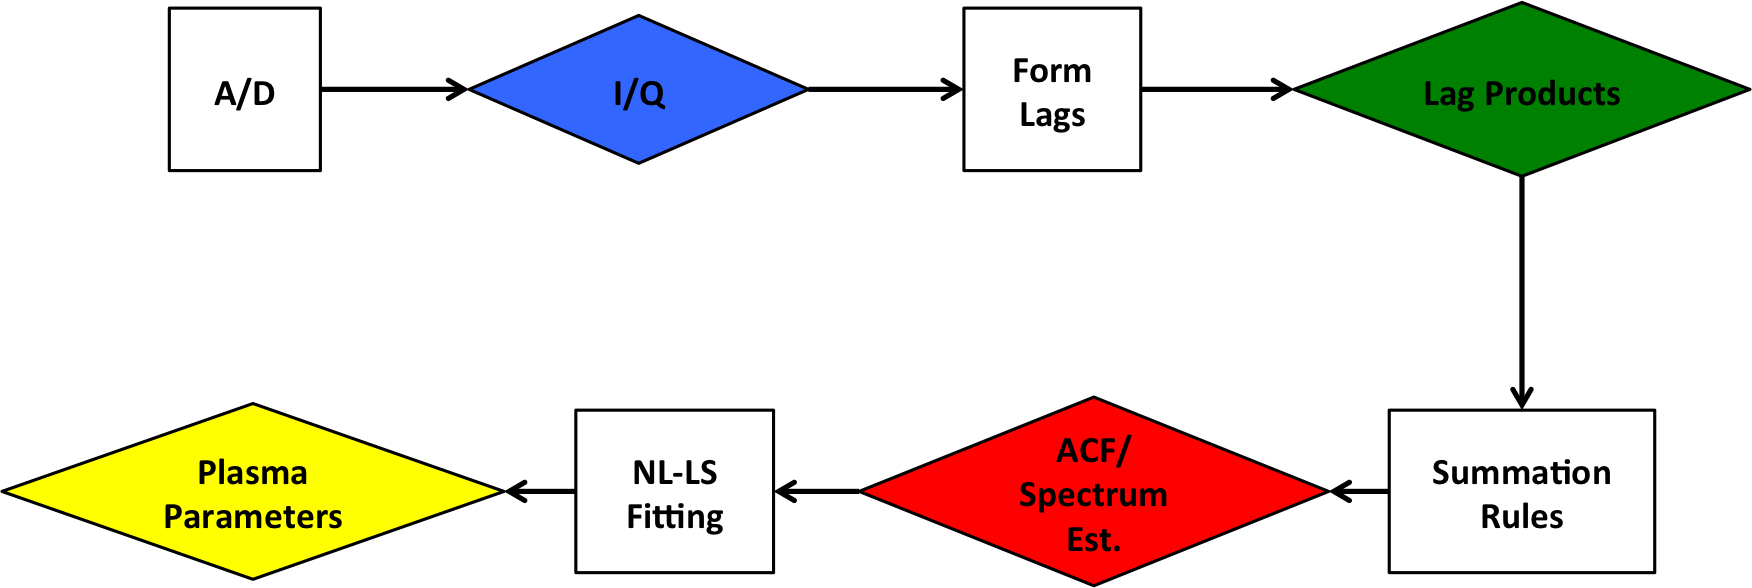
\includegraphics[width=6in]{datastackchain}
\caption{ISR signal processing chain, with signal processing operations as squares and data products as diamonds.}
\label{fig:chain}
\end{figure}



\section{Lag Product Formation}
The lag product formation is an initial estimate of the autocorrelation function. The sampled I/Q can be represented as $x(n) \in\mathbb{C}^N$ where $N$ is the number of samples in an inter pulse period. For each range gate $m\in 0,1,...M-1$ an autocorrelation is estimated for each lag of $l \in 0,1...,L-1$.  To get better statistics this operation is performed for each pulse $j\in 0,1,...J-1$ and then summed over the $J$ pulses. The entire operation to form the initial estimate of $\hat{R}(m,l)$ can be seen in Equation \ref{lagpro}:

\begin{equation}
\label{lagpro}
\hat{R}(m,l) = \displaystyle\sum\limits_{j=0}^{J-1} x(m-\lfloor l/2\rfloor,j)x^*(m+\lceil l/2 \rceil,j).
\end{equation}

The case shown in Equation \ref{lagpro} is a centered lag product, other types of lag products calculations are available but generally a centered product is used. In the centered lag product case range gate index $m$ and sample index $n$ can be related by $m=n-\lfloor L/2\rfloor$ and the maximum lag and sample relation is $M=N-\lceil L/2 \rceil$.  This lag product formation is the first step in taking a discrete Wigner Distribution \cite{TFAcohen}.

This specific type of lag product formation is detailed in \cite{farley1969} and had been referred to as unbiased. This terminology does differ from what is used in statistic signal processing literature such as \cite{randomsigshanmugan} where the unbiased autocorrelation function estimate is carried out as so,

\begin{equation}
\label{eq:lagproub}
\hat{R}(m,l) = \frac{1}{L-l}\displaystyle\sum\limits_{j=0}^{J-1} x(m-\lfloor l/2\rfloor,j)x^*(m+\lceil l/2 \rceil,j).
\end{equation}

\noindent With out the $\frac{1}{L-l}$ term the estimator will be windowed with a triangular function thus impacting the estimate of the ISR spectrum as this will act as a convolution in the frequency domain. This bias is taken into account in \cite{farley1969} but it is simply wrapped up into the ambiguity function. 

\section{Summation Rules}
Applying a summation rule is usually the next step in creating an estimate of the autocorrelation function.  This is done to get a constant range ambiguity across all of the lags for long pulse experiment\cite{nygren1996}. It also equalizes the statistics for each lag as the higher lags have greater variance. 

An example summation rule for a forward product is shown in Figure \ref{fig:sumrule}. In the figure the image on the left is a basic representation of an ambiguity function of a long pulse.  Its mirrored on the right with red bars which would show the integration area under it so the ambiguity function will be of equal size in range.  

In the processing this is basically a summing of lags from different ranges.  The amount of summing is similar to what is shown in Figure \ref{fig:sumrule}.  There are a number of different summing rule each with their own trade offs \cite{nygren1996}.  

Lastly an estimate of the noise correlation is subtracted out of $\hat{R}(m,l)$, which is defined as $\hat{R}_w(m,l)$:

\begin{equation}
\label{lagpro}
\hat{R}_w(m,l) = \displaystyle\sum\limits_{j=0}^{J-1} w(m_w-\lfloor l/2\rfloor,j)w^*(m_w+\lceil l/2 \rceil,j),
\end{equation}

\noindent where $w(n_w)$ is the background noise process of the radar.  Often the noise process is sampled during a calibration period for the radar when nothing is being emitted.  The final estimate of the autocorrelation function after the noise subtraction and summation rule will be represented by $\hat{R}_f(m,l)$.
\begin{figure}[!t]
\centering
\includegraphics[width=3in]{sumrule}
% where an .eps filename suffix will be assumed under latex, 
% and a .pdf suffix will be assumed for pdflatex; or what has been declared
% via \DeclareGraphicsExtensions.
\caption{Summation Rule Diagram}
\label{fig:sumrule}
\end{figure}

\section{Nonlinear Least-Squares Fitting}
After the final estimation of the spectrum is complete the nonlinear least squares fitting takes place to determine the parameters.  The basic class of nonlinear least-squares problems as seen in \cite{kayvol1}, are shown in Equation \ref{nlls},

\begin{equation}
	\hat{\mathbf{p}}= \underset{\mathbf{p}}{\text{argmin}} (\mathbf{y}-\bm{\theta}(\mathbf{p}))\bm{\Sigma}(\mathbf{y}-\bm{\theta}(\mathbf{p}))^*.
\label{nlls}
\end{equation}

In Equation \ref{nlls}, the data represented as $\mathbf{y}$ would be the final estimate of the autocorrelation function $\hat{R}_f(m,l)$ at a specific range or its spectrum $\hat{S}_f(m,\omega)$.  The parameter vector $\mathbf{P}$ would be the plasma parameters $N_e$, $T_e$, $T_i$ and various other parameters including ion velocities. The fit function $\bm{\theta}$ is the IS spectrum calculated from models, such as once seen in \cite{kudeki:milla:1}, smeared by the ambiguity function.  In the case of the long pulse the ambiguity can be simply applied by multiplying it with the autocorrelation function $R(l)$, if the summation rule is properly applied.  Lastly the correlation matrix $\bm{\Sigma}$ if often realized as a diagonal matrix for many ISR systems.  If it was not that would imply correlation with the measurement uncertainties between different lags or samples of the spectrum.  The diagonal values usually used, noted as $\sigma_i^2$, usually the same unless there is a larger measurement error for one of the lags or spectrums.  The following formula from  \cite{nicollsisrschool2013} can be used:

\begin{equation}
\label{sigpow}
\sigma_i = \frac{S}{\sqrt{J}}\left(1+\frac{1}{SNR}\right).
\end{equation}

\noindent where $S$ is the signal power and $SNR$ is the signal to noise ratio.  These quantities can be estimated using the calibration period.


In the past ISR researchers have used the Levenberg-Marquart algorithm to fit data \cite{nikoukar2008}.  This specific iterative algorithm moves the parameter vector $\mathbf{p}$ by a perturbation $\mathbf{h}$ at each iteration\cite{gavin:2013}.  Specifically Levenberg-Marquart was designed to be a sort of meld between two different methods Gradient Decent, and Gauss-Newton.  The perturbation vector $\mathbf{h}_{lm}$ can be calculated using the following:

\begin{equation}
\left[ \mathbf{J}^T\bm{\Sigma}\mathbf{J}\right]\mathbf{h}_{lm} =\mathbf{J}^T\bm{\Sigma}(\mathbf{y}-\bm{\theta})
\label{hlm}
\end{equation}

\noindent where $\mathbf{J}$ is the Jacobian matrix $\partial \bm{\theta}/\partial \mathbf{p}$ \cite{levenberg1944} \cite{marquardt:1963}


 \bibliographystyle{BibTeX/ieeetrsrt}

 \bibliography{BibTeX/litreview}

 \end{document}